\chapter{Write Error Rate measurement}

In order to make magnetic tunnel junctions as the cell for future Magnetic Random Access memory, it is important to characterize the switching property for MTJs, which setting the MTJs to a desired state(write). This measurement is known as the Write Error Rate(WER). Formally, applying the electric pulse at different duration and amplitude, by monitoring the resistance before and after the pulse, we can find the switching probability. For optimizing the WER, we need to consider the power consumption and also the switching time. Moreover, from a fundamental physical point of view, it is important to understand the detailed switching mechanism. In the previous chapter, we have already shown how to observe switching in time-domain. 

The Write Error Rate(WER) is defined as the ratio between number of non-switching attempt with the total switching attempt. So WER can be understood as the probability of not successful attempt. The typical error used in common computer memory is around $10^{-9}$. Therefore, in order to reliably characterize the WER, we need to obtain very large statistics, which is only increasing by taking into account the approximately $\sqrt{N}$ counting error associated with the binary results of a switching attempt. It would take years by employing conventional DC resistance measurement in this sense. To overcome this, we are going to a quick and accurate measurement of WER with large statistics as a function of certain parameters.

\section{Experimental Setup}

We first show the experiment set-up for write error rate measurement\ref{fig:WER}. As we can see, the circuit has been divided into two parts. In the AC part, a Picosecond Pulse Labs 10,0070A pulse generator (PSPL) is used to generate write pulses and an Agilent 33220A Arbitrary Waveform Generator (ARB) provides the reset pulse. We then use a Keithley 2400 source Meter(Keithley) to provide a small DC bias voltage, which will then be National Instruments USB-6251 BNC Digital Acquisition Board (DAQ)

\begin{figure}[h!]
    \centering
    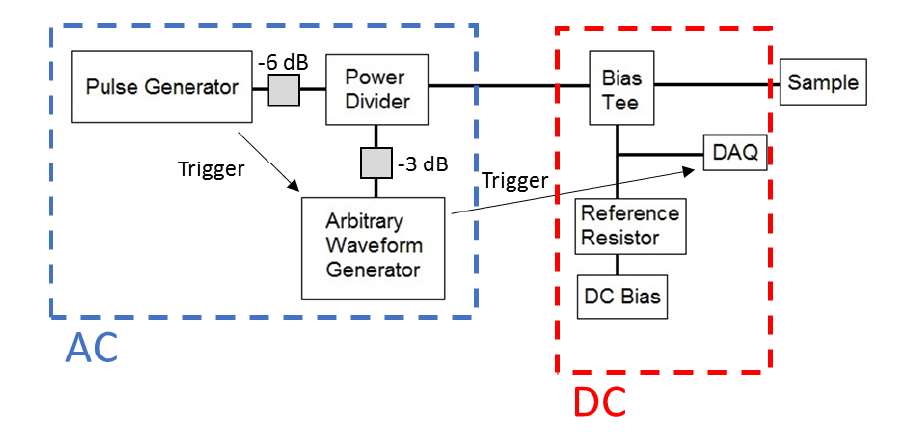
\includegraphics[width=1.0\textwidth]{fig/WER_setup.PNG}
    \caption{Write Error Rate measurement set-up, here we include AC and DC circuit}
    \label{fig:WER}

\end{figure}

The PSPL can provide pulses from 100 picosends to 10 nanoseconds, while the ARB has a pulse range from 50 nanoseconds to DC. Our goal is to generate a pulse sequence as it is shown in \ref{fig:Pulse}.

\begin{figure}[h!]
    \centering
    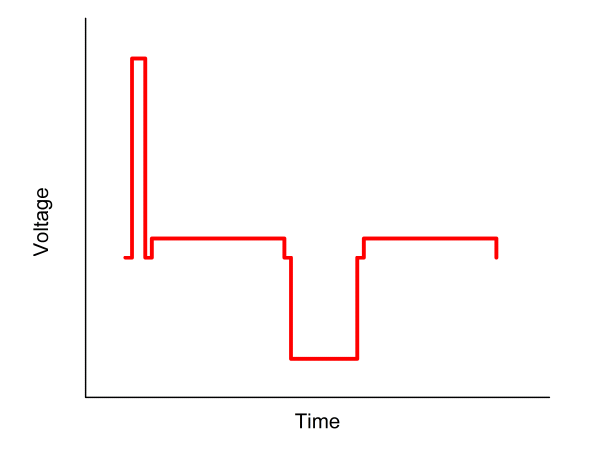
\includegraphics[width=0.5\textwidth]{fig/pulse.PNG}
    \caption{Pulse shape used in Write Error Rate Measurement}
    \label{fig:Pulse}
\end{figure}




In order to produce such a pulse sequence, we need to establish correct synchronization. To do that, the following procedure has been carried out:

1. Connect the trigger output of the PSPL to the trigger input of the ARB. This port of the ARB is labeled Ext. Trig., which is located
on the rear panel.

2. Set the PSPL trigger method to Internal with a repetition rate appropriate for the
length of pulse train used (for the work presented in this thesis, 2.5 kHz was used). Now the PSPL is used to control the remaining instruments

3. Set the ARB trigger to Ext. Trig. (rising edge) and the output mode to Burst. This will allow the ARB to generate a bust of pulse sequence once tiggered. 

4. Connect the trigger output of the ARB (labeled ”Sync”) to the trigger input of the DAQ, labeled APFI0 (analog programmable function interface) for the model mentioned above.

5. Set the DAQ trigger to APFI0 and the sampling rate to maximum (1.25 MSamples/s in the case of this DAQ)

6. Connect a reference resistor to the DC bias and then connect it to the DC port of the bias tee. Usually this reference resistor should have resistance in the middle of parallel and anti-parallel state. The DC bias should have constant output and is chosen to have a polarity to favor the switched state.

7. Connect an analog input of the DAQ (any will do) between the reference resistor and the bias tee.

8. Connect the outputs of the PSPL and ARB, with appropriate attenuators to protect the equipment at the hardware level (for the equipment and circuit used here, -6 dB and -3 dB respectively), to the power divider. Then connect the remaining port of the power divider to the AC port of the bias tee. All connection cables used should be rated for the appropriate frequency of the pulses.

The logical behind the experiment setup is explained the following. To measure the switching probability at a fixed pulse, we need to record the resistance before the pulse and after the pulse. Clearly, it would not be practicable to measure the resistance using a Keithley(it would be painfully slow). By inserting a reference resistor between the sample and DC source, the voltage passing through the reference resistor would change according to the sample resistance. By recording the voltage in real time, we can record the resistance of the sample.

Another import aspect of the measurement is to properly reset the state. Of course, using a magnetic field to reset is not acceptable. To accomplish that, we use ARB to generate a opposite pulse as write pulse. To save the sample from electrical breakdown, the reset pulse is usually longer than write pulse and should have relatively low amplitude.

The raw data we get from the automation software such as LabView would be a voltage trace of many switching attempts. Usually LabView is not efficient enough to handle such a great amount of data. So we choose to have LabView to extract two sections of each switch attempt corresponding to the read pulse and write pulse. This method will give us a long list of initial and final voltages from each switching attempt that can be then translate into resistance and then compare to evaluate the success of each switching attempt.

Given the voltage recorded by the DAQ, we can convert the voltage to resistance of the sample. The DC part of the circuit is a voltage divider, the resistance of the MTJ as a function of the measured DAQ voltage $V_{\mbox{DAQ}}$ is given by
\begin{equation}\label{eq:1}
\centering
R_{\mbox{MTJ}} = \frac{R_{\mbox{Ref}}V_{\mbox{DAQ}}}{V_{\mbox{DAQ}}- V_{\mbox{Read}}}
\end{equation}

where$R_{\mbox{Ref}}$ is the value of the reference resistor and $V_{\mbox{Read}}$ is the read voltage. Here the value of $V_{\mbox{Read}}$ should be properly picked. The read voltage should be higher enough to well separate two states, at the same time, higher read voltage would disturb the switching state. To show that, the voltage difference between anti-parallel state and parallel state is the following:

\begin{equation}\label{eq:2}
\centering
\Delta V_{\mbox{DAQ}} = V_{\mbox{read}} \frac{(R_{\mbox{AP}}R_{\mbox{Ref}}- R_{\mbox{P}}R_{\mbox{Ref}})}{(R_{\mbox{AP}} +  R_{\mbox{Ref}})(R_{\mbox{P}} -  R_{\mbox{Ref}})}
\end{equation}
where $R_{\mbox{AP}}$ and $R_{\mbox{P}}$ are anti-parallel and parallel resistance of the device. Here we find that the voltage difference is linearly depend on the read voltage.

Now we have to determine an adequate and safe reset voltage and process the raw data output by LabView. One first needs to process some initial data and then optimize based upon the results in an iterative fashion to assess the efficiency of the reset pulse. To analyze the raw data file, a python script carry out the following routine:

1. Read the raw data file and extract all initial and final measured voltage(before and after pulse.)

2. Convert the raw voltage into resistace using Equation\ref{eq:2}.  

3. Determine the device state for each voltage value. This can be done by considering the known parallel and anti-parallel states. Usually, if the read voltage is positive, the AP state should have higher voltage.

4. Compare initial and final voltage for each switching attempe and categorize into three possible cases: switched(the device starts in the correct state and ended in the opposite state), not-switched(the device starts in the correct state and fail to switch), and missed(the device starts at the wrong state.)

5. Sum over all the switching attempt. The write error rate is given as $\frac{N_{NotSwitched}}{N_{attempts}-N_{missed}}$

To determine the necessary reset voltage, we adapt the following iterative process:

1. Set the write voltage so that most of the switching attempts are successful.

2. Set the reset voltage to a safe and small amount. A good starting point is half of the write voltage.

3. Start the measurement and process the data. Identify the number of missed events, which means the device has not been set properly to the desired initial state.

4. Slowing increase the reset voltage so that the number of missed event is much less than one per cent of the total switching events.

Since the duration of the reset pulses are much longer than write pulses(typical resets pulse duration are 100~500 ns while write pulses are usually smaller than 10 ns). The proper value of reset pulse is very important for this measurement. If the reset pulse is too small, then many of switching attempts would not be used in the final data analysis. If the reset pulse is too large, then we take the risk of device breakdown. Now with our measurement technique explained, we can reliably and efficiently study Write Error Rate as a function of write pulse and voltage, applied magnetic field or any other interesting parameters. With our experimental set-up, $10^6$ switching attempts can be completed in 8.5 minutes.


\section{Results and Discussion}
Detailed switching mechanism by applying the spin transfer torque is still unclear. People have argued that it is possible some sub-area will act as an activation regime which will leads the switching\cite{Sub}. It is proposed that at finite temperature, switching probability is proportional to applied voltage\cite{Sun1991}. However recently people have found anomalous behavior at certain amplitude and polarity\cite{Back-hopping}\cite{High_bias}\cite{BitError}. We would like to test the switching probability measurement on our samples.

\begin{figure}[h!]
    \centering
    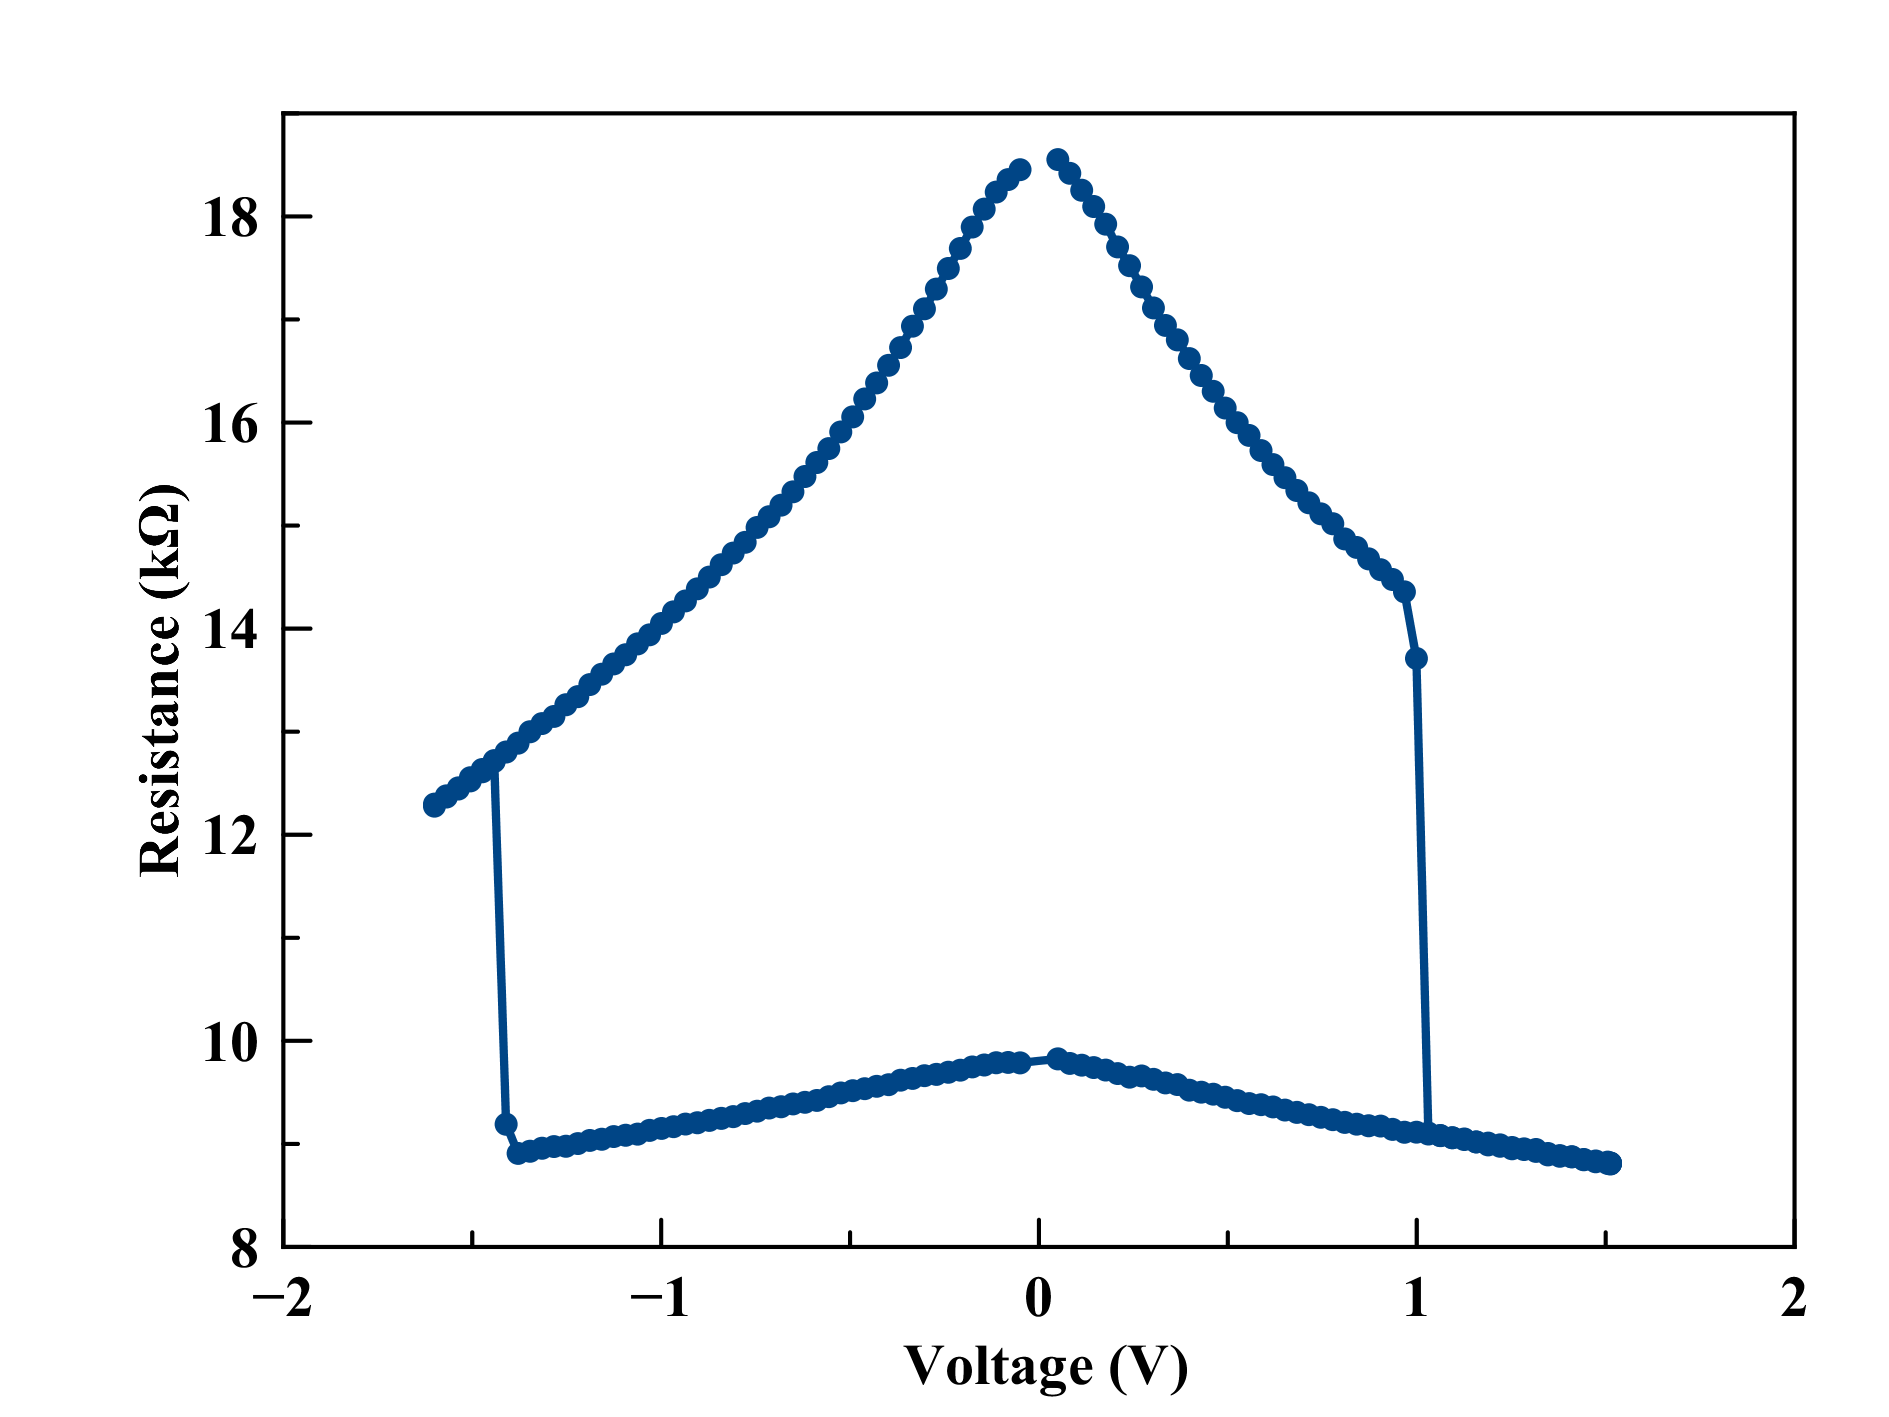
\includegraphics[width=0.5\textwidth]{fig/mr.png}
    \caption{Resistance versus dc voltage at zero magnetic field}
    \label{fig:mr_wer}
\end{figure}

Before we make Write Error Rate measurement, we need to measure the resistance as a function of dc voltage to identify the switching probablity. Fig.\ref{fig:mr_wer} shows one example of sample resistance as a function of applied dc voltage. At positive polarity, the device starts at high-resistance(anti-parallel)state. The resistance drops with increasing voltage. Around 1 V, the resistance drops to low-resistance(parallel)state and stay at parallel state when the voltage keep increasing. Now if we keep the device to be in the parallel state and start to apply the negative voltage, around negative 1.5 V, the resistance of the device will go up, which means switching from parallel to anti-parallel. So from this curver we know that by applying the postive voltage pulse, we can switch the device from anti-parallel state to parallel state.

To perform the write error rate measurement, we first initialize the device at the anti-parallel state using magnetic field, then we constantly apply the positive voltage as we dicussed in the previous section. Appropriate reset voltage has been chosen to reset the device back into anti-parallel state. In this set-up of measurement we fix the pulse duration to be 10 ns and only varying the pulse amplitude. The result is shown in Fig.\ref{fig:wer_1}

\begin{figure}[h!]
    \centering
    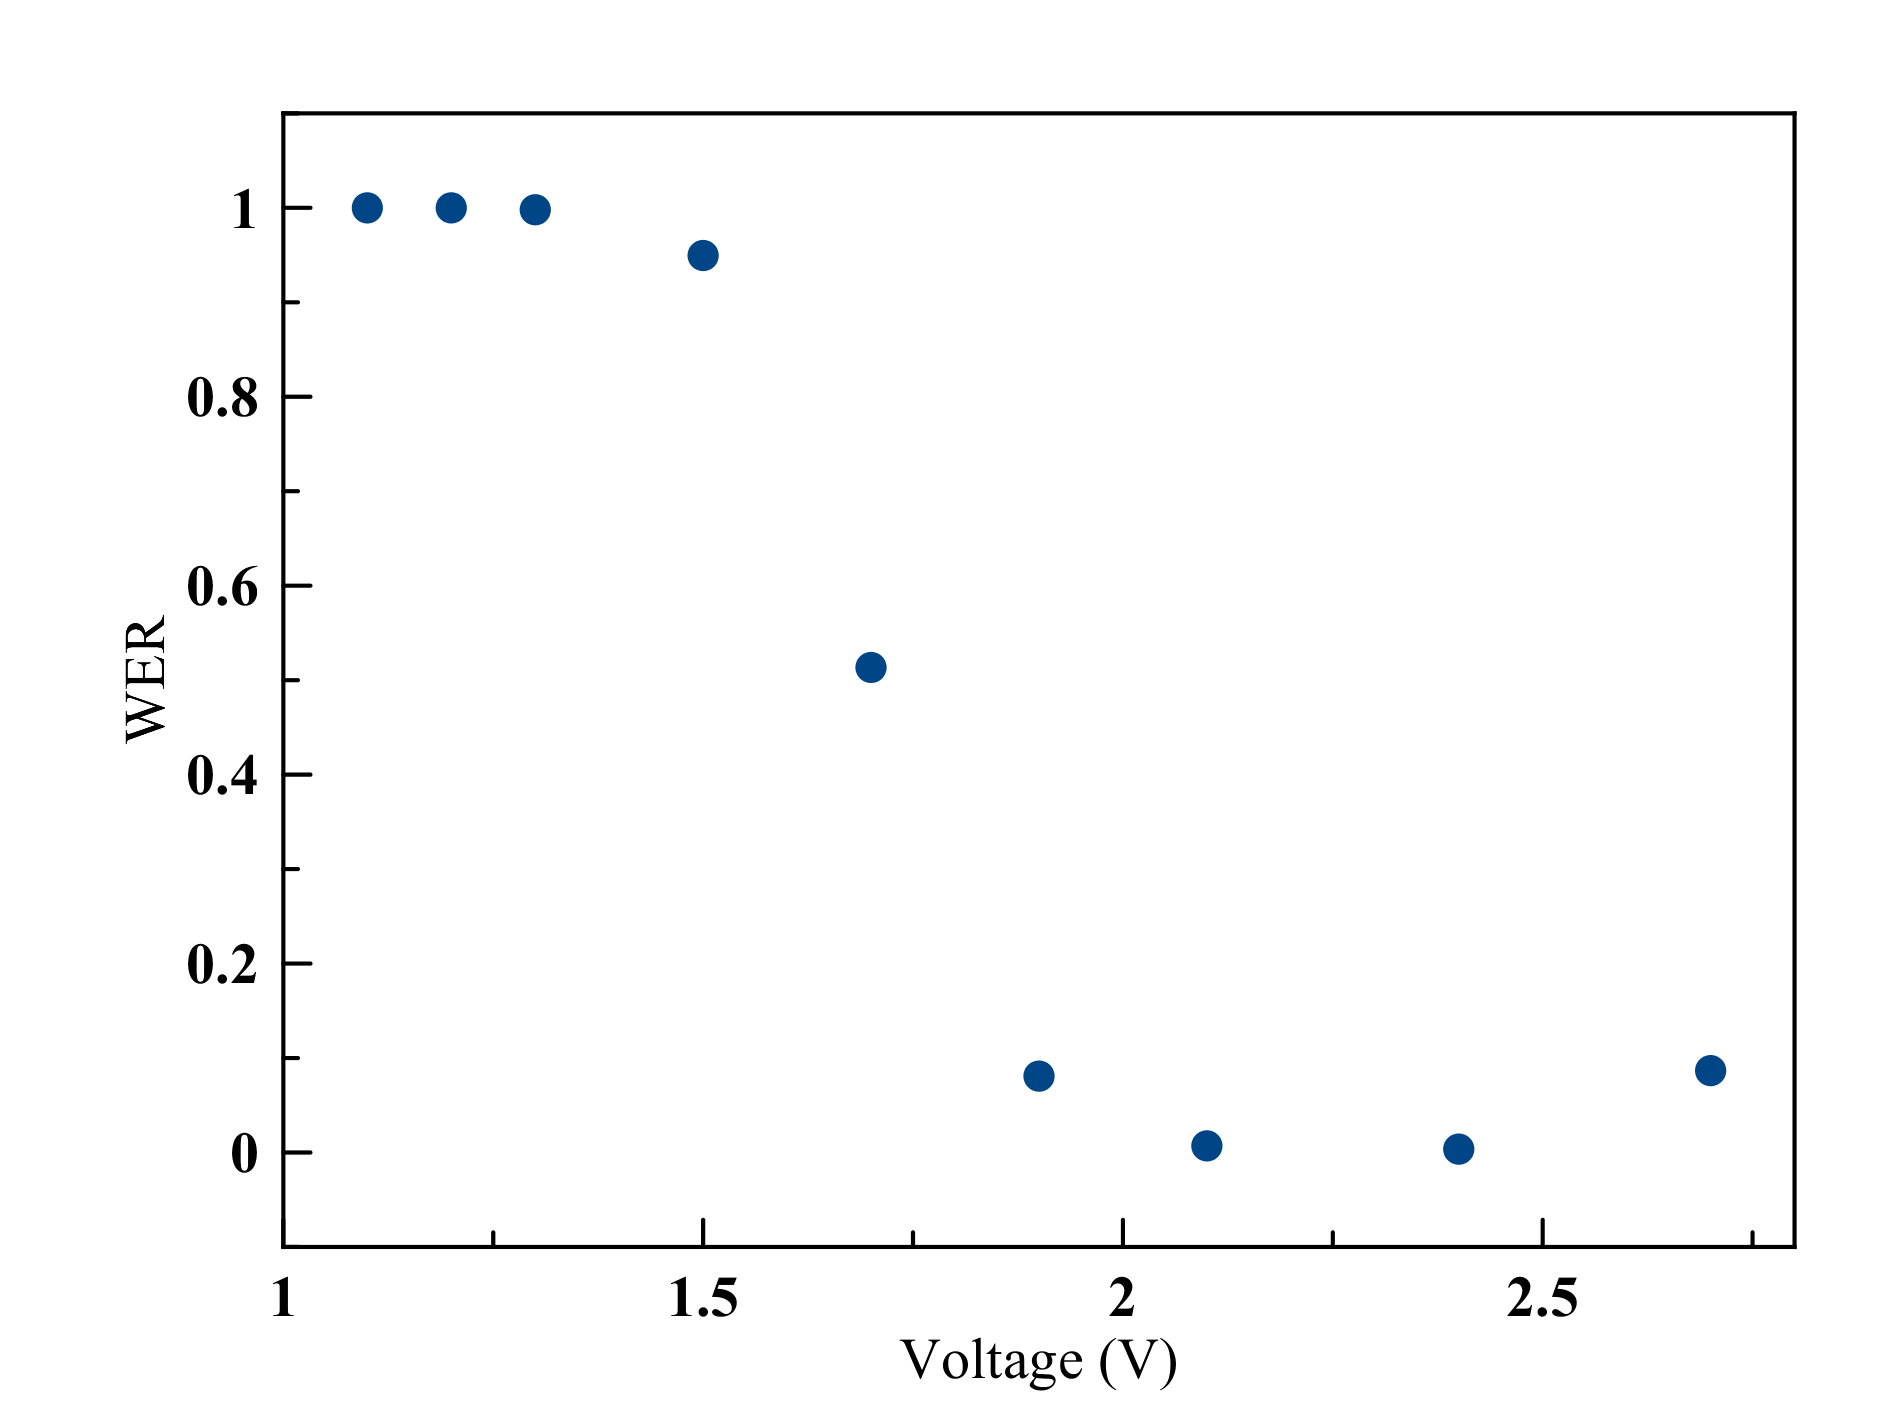
\includegraphics[width=0.5\textwidth]{fig/wer_1.png}
    \caption{Write Error Rate curve for one typical device studied in the experiment.}
    \label{fig:wer_1}
\end{figure}

At low amplitude pulse, the switching probability is indeed very low, close to zero. As we gradually increase the pulse amplitude, around 1.5 V, the device start to increase and the WER is close to zero at around 2 V applied voltage. So far everything is as expected. However, starting from 2 V when we would normally expect the WER to keep decreasing at increasing applied voltages, we find that however, the WER start to increase somehow. More formally, from a uniform switching theory, the WER should have Gaussian dependence with respect to voltage at finite temperature\cite{Back-hopping}, so we can call this non-Gaussian behavior to be anomalous WER.

Different mechanism has been proposed to explain the anomalous WER behavior. One possible origin is coming from non-linear coupling between modes excited in MTJs \cite{Correlation}\cite{Para}. Another suspect is the formation of sub-volume domain in the switching process. Previously, people believe that the switching process is dominate by sub-volume switching\cite{subswitch}\cite{Sub}. However now there is a growing evidence to show that the Dzyaloshinskii-Moriya interaction can significantly affect the switching process and cause the meta-stable state which is unfavorable for switching\cite{DMI}.






%\begin{figure}[h!]
 %   \centering
  %  \includegraphics[width=0.5\textwidth]{fig/wer_2.png}
   % \caption{Pulse shape used in Write Error Rate Measurement}
   % \label{fig:wer_2}
%\end{figure}